\chapter{Methods}
\section{Water Year 2019} 
\subsection{Temperature Array}
Our temperature sensor is located at Banner Creek Summit in central Idaho. This location has an elevation of about 7,040 feet above sea level and is off of Idaho State Highway 21. The area around Banner Summit receives an average of 1.9 meters of snow each year and frequently experiences extreme low temperatures as low as -40\textdegree C. The 2018 -- 2019 winter season was above average with a peak snow water equivalent (SWE) measured at Banner Summit at 120\% of average. Site visits occur on a biweekly basis unless weather or road closures forbid access. During each visit, data is collected from the instrument and snow samples are collected for stable water isotope analysis.

The structure of our sensor is comprised of a steel, rectangular frame with thin, metal cables running horizontally in 5cm increments (Fig. \ref{fig:Banner_Sensor}). Omega Type T thermocouples are attached to each wire which forms a vertical array of temperature sensors up to 2.5m above the ground. There are two thermocouples buried in the soil at 10cm and 5cm below ground. The buried 10cm thermocouple is installed directly adjacent to a thermistor (Campbell Scientific T107). The 53 thermocouples are multiplexed using a Campbell Scientific AM32 to a Campbell Scientific CR1000 data logger. Temperature measurements are recorded every 5 minutes. The design for this sensor came from Charlie Luce and Tom Black at the USFS and it is based off an existing sensor currently installed at Bogus Basin, outside of Boise. 

A Micro-Specialties Irridium Satellite telemetry system was installed during the 2020 water year so that data are accessible in near-real time. Data is transmitted every six hours using an hourly average from the measurements taken the hour before each transmit. This data is ingested using a python script that visualizes and does statistical analysis on the incoming data. [Reference?] 

 \begin{figure}[!t]
    \centering
    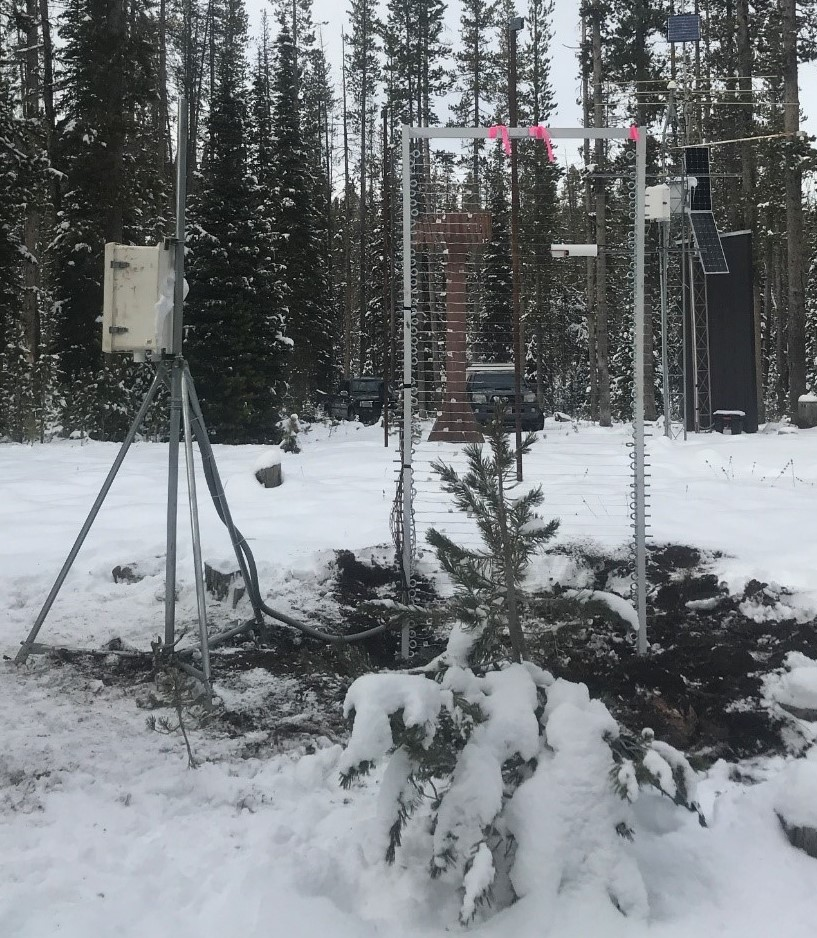
\includegraphics[width=0.8\linewidth]{figures/Banner_Sensor.jpg}
    \caption{Picture of the instrument installed at Banner Creek Summit.}
    \label{fig:Banner_Sensor}
 \end{figure}

\subsection{Stable Water Isotopes}
Snow was sampled within 20 meters of the Banner Summit SNOTEL site for analysis of stable water isotopes. The snow pit locations are randomly selected on a flat surface with no apparent aspect. The sampled area is lightly forested, but care is taken in order to prevent contamination from secondary snow input such as fallen, intercepted snow or wind drifts. In order to capture the full isotopic content of a snowpack, samples are collected from the whole snow profile with a 3cm vertical resolution. To assess spatial variability of stable water isotopes, duplicate samples were collected from one pit with about 0.5 m horizontal spacing (figure \ref{fig:Pit_18Dec19}). To assess systematic bias in the sampling method, samples were collected in triplicates directly adjacent to each other (figure \ref{fig:Pit_17Mar19}). Detailed notes are taken on snowpack characteristics during each sampling event.

 \begin{figure}[!t]
    \centering
    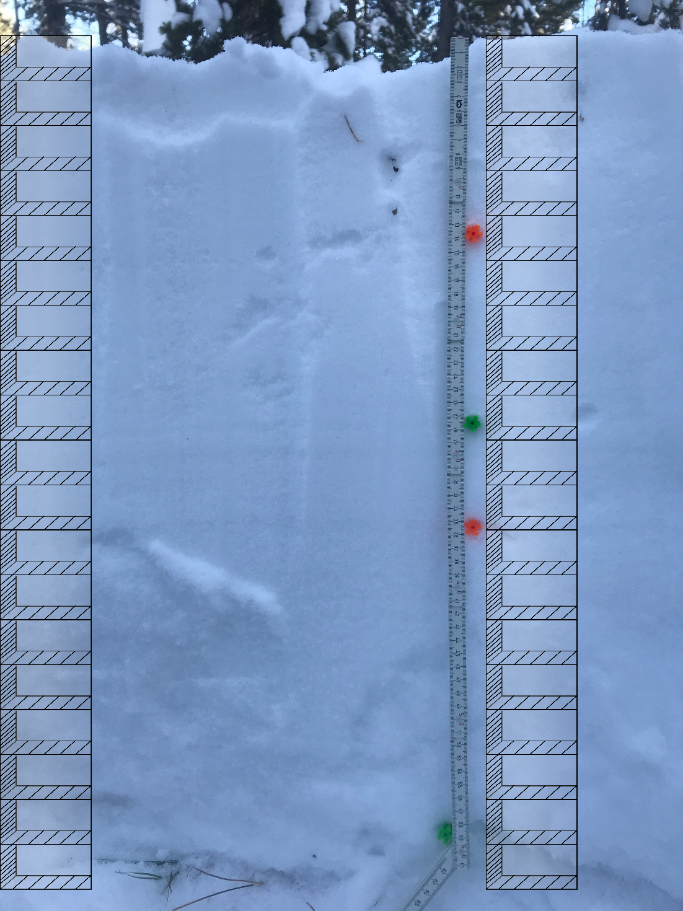
\includegraphics[width=0.5\linewidth]{figures/Pit_18Dec19.png}
    \caption{Picture of the sampling method used on December 18, 2018 showing duplicates taken with about 0.5m spacing.}
    \label{fig:Pit_18Dec19}
 \end{figure}
 
 \begin{figure}[!t]
    \centering
    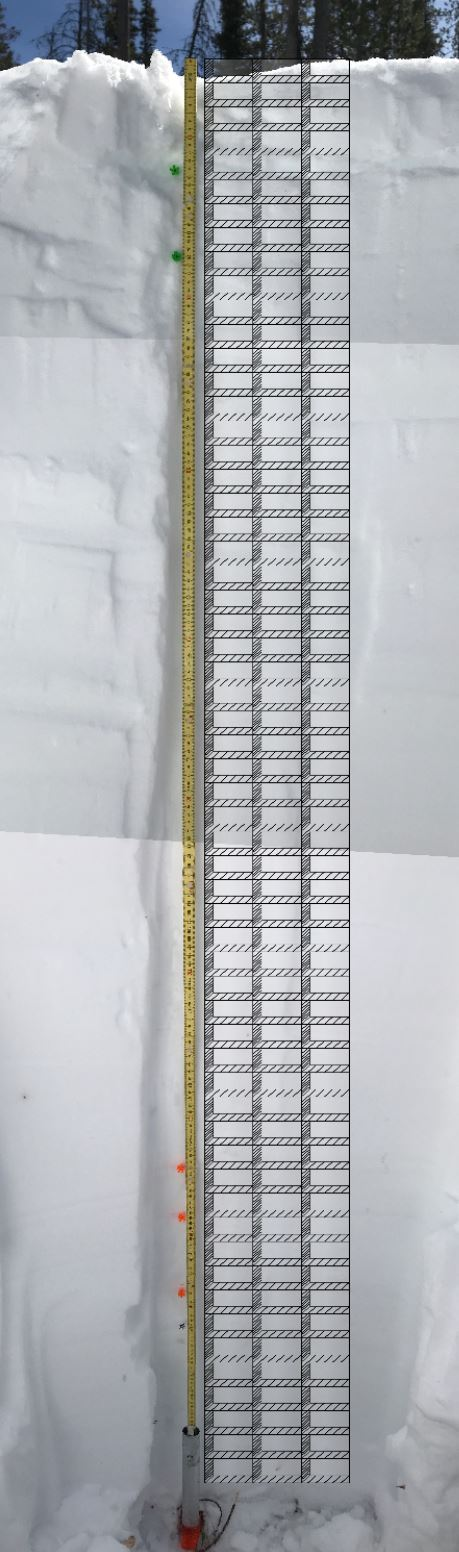
\includegraphics[width=0.3\linewidth]{figures/Pit_17Mar19.jpg}
    \caption{Picture of the sampling method used on March 17th, 2019 showing triplicates taken directly adjacent to each other.}
    \label{fig:Pit_17Mar19}
 \end{figure}

Snow samples are transported back to Boise State where they are stored at -20°C. A fourth generation Los Gatos Research (LGR) Liquid Water Isotope Analyzer (LWIA) is used to measure \textsuperscript{2}H/\textsuperscript{1}H and \textsuperscript{18}O/\textsuperscript{16}O for all snow samples. Results are reported in units of per mil (\textperthousand), relative to Vienna Standard Mean Ocean Water (VSMOW). Raw LWIA values are processed using the Los Gatos Research post-processing software.